\documentclass{standalone}
\usepackage{tikz}
\usetikzlibrary{patterns, positioning}
\usetikzlibrary{shapes.misc}
\usepackage[outline]{contour}
\contourlength{1.5pt} 


\begin{document}
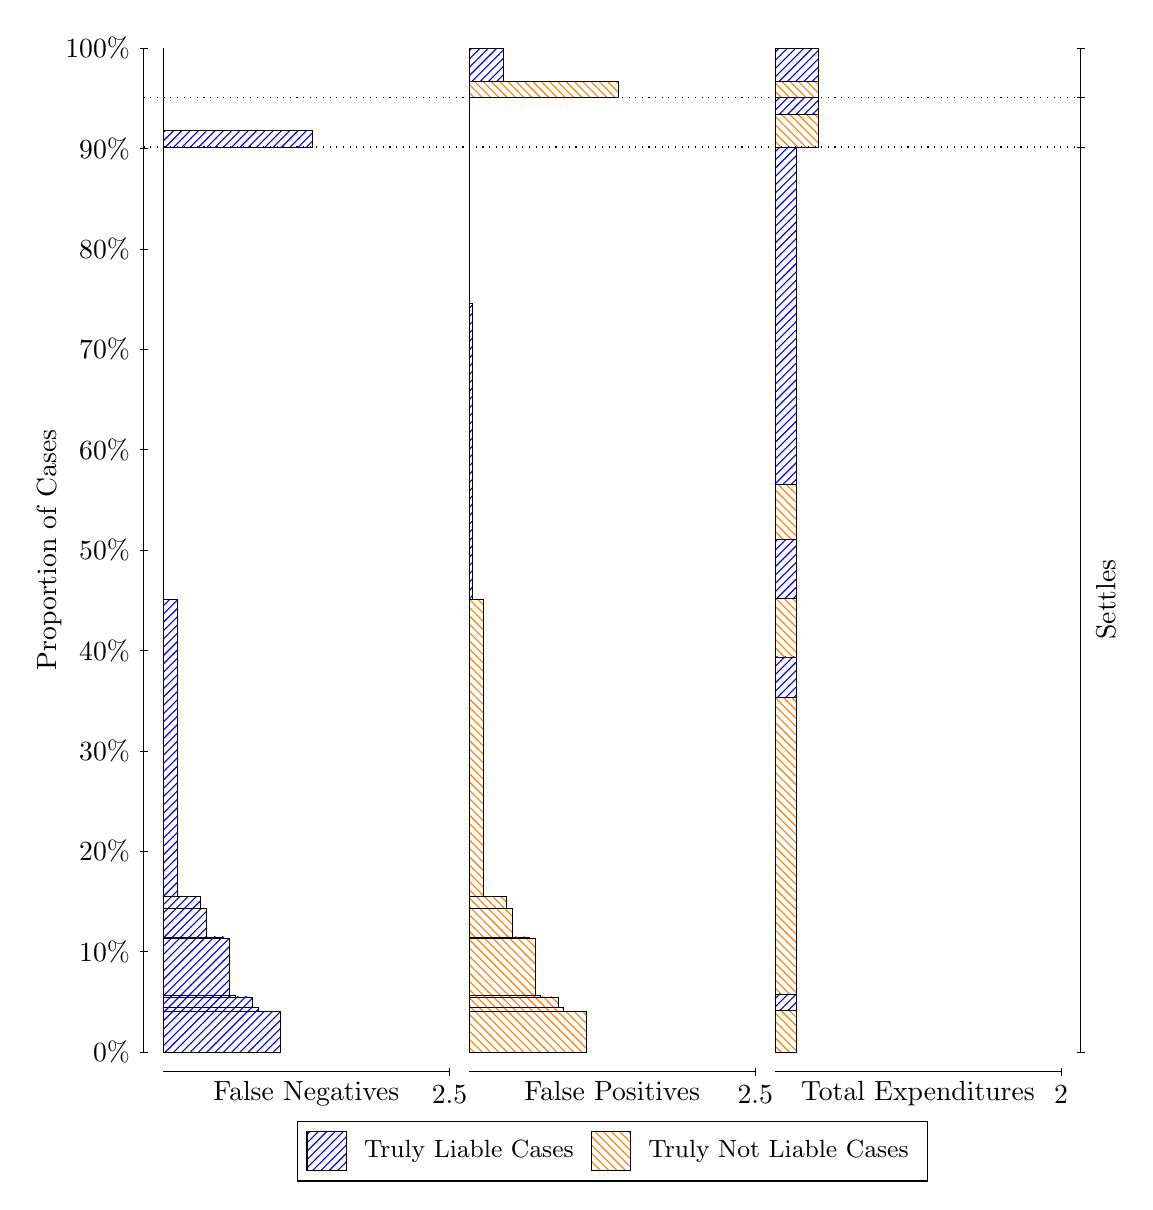
\begin{tikzpicture}
\draw[black, very thin] (1.5,1.75) -- (1.5,14.5);
\node[rotate=90, text=black, anchor=center] at (0.3, 8.125) {Proportion of Cases};
\draw[black, very thin] (1.45,1.75) -- (1.55,1.75);
\node[text=black, anchor=east] at (1.45, 1.75) {0\%};
\draw[black, very thin] (1.45,3.025) -- (1.55,3.025);
\node[text=black, anchor=east] at (1.45, 3.025) {10\%};
\draw[black, very thin] (1.45,4.3) -- (1.55,4.3);
\node[text=black, anchor=east] at (1.45, 4.3) {20\%};
\draw[black, very thin] (1.45,5.575) -- (1.55,5.575);
\node[text=black, anchor=east] at (1.45, 5.575) {30\%};
\draw[black, very thin] (1.45,6.85) -- (1.55,6.85);
\node[text=black, anchor=east] at (1.45, 6.85) {40\%};
\draw[black, very thin] (1.45,8.125) -- (1.55,8.125);
\node[text=black, anchor=east] at (1.45, 8.125) {50\%};
\draw[black, very thin] (1.45,9.4) -- (1.55,9.4);
\node[text=black, anchor=east] at (1.45, 9.4) {60\%};
\draw[black, very thin] (1.45,10.675) -- (1.55,10.675);
\node[text=black, anchor=east] at (1.45, 10.675) {70\%};
\draw[black, very thin] (1.45,11.95) -- (1.55,11.95);
\node[text=black, anchor=east] at (1.45, 11.95) {80\%};
\draw[black, very thin] (1.45,13.225) -- (1.55,13.225);
\node[text=black, anchor=east] at (1.45, 13.225) {90\%};
\draw[black, very thin] (1.45,14.5) -- (1.55,14.5);
\node[text=black, anchor=east] at (1.45, 14.5) {100\%};

\draw[black, very thin] (13.4,1.75) -- (13.4,14.5);
\draw[black, very thin] (13.35,1.75) -- (13.45,1.75);
\node[anchor=west] at (13.35, 1.75) {};
\draw[black, very thin] (13.35,13.243) -- (13.45,13.243);
\node[anchor=west] at (13.35, 13.243) {};
\draw[black, very thin] (13.35,13.872) -- (13.45,13.872);
\node[anchor=west] at (13.35, 13.872) {};
\draw[black, very thin] (13.35,14.5) -- (13.45,14.5);
\node[anchor=west] at (13.35, 14.5) {};

\draw[black, very thin, pattern color=blue, pattern=north east lines] (1.75,1.75) rectangle (3.2397,2.2619);
\draw[black, very thin, pattern color=blue, pattern=north east lines] (1.75,2.2619) rectangle (2.949,2.3206);
\draw[black, very thin, pattern color=blue, pattern=north east lines] (1.75,2.3206) rectangle (2.8763,2.4499);
\draw[black, very thin, pattern color=blue, pattern=north east lines] (1.75,2.4499) rectangle (2.6583,2.4658);
\draw[black, very thin, pattern color=blue, pattern=north east lines] (1.75,2.4658) rectangle (2.5857,3.1962);
\draw[black, very thin, pattern color=blue, pattern=north east lines] (1.75,3.1962) rectangle (2.513,3.2121);
\draw[black, very thin, pattern color=blue, pattern=north east lines] (1.75,3.2121) rectangle (2.295,3.569);
\draw[black, very thin, pattern color=blue, pattern=north east lines] (1.75,3.569) rectangle (2.2223,3.7308);
\draw[black, very thin, pattern color=blue, pattern=north east lines] (1.75,3.7308) rectangle (1.9317,7.4966);
\draw[black, very thin, pattern color=orange, pattern=north west lines] (1.75,7.4966) rectangle (1.75,13.243);
\draw[black, very thin, pattern color=blue, pattern=north east lines] (1.75,13.243) rectangle (3.6393,13.451);
\draw[black, very thin, pattern color=orange, pattern=north west lines] (1.75,13.451) rectangle (1.75,13.872);
\draw[black, very thin, pattern color=orange, pattern=north west lines] (1.75,13.872) rectangle (1.75,14.08);
\draw[black, very thin, pattern color=blue, pattern=north east lines] (1.75,14.08) rectangle (1.75,14.5);
\draw[black, very thin, pattern color=orange, pattern=north west lines] (5.6333,1.75) rectangle (7.123,2.2619);
\draw[black, very thin, pattern color=orange, pattern=north west lines] (5.6333,2.2619) rectangle (6.8323,2.3206);
\draw[black, very thin, pattern color=orange, pattern=north west lines] (5.6333,2.3206) rectangle (6.7597,2.4499);
\draw[black, very thin, pattern color=orange, pattern=north west lines] (5.6333,2.4499) rectangle (6.5417,2.4658);
\draw[black, very thin, pattern color=orange, pattern=north west lines] (5.6333,2.4658) rectangle (6.469,3.1962);
\draw[black, very thin, pattern color=orange, pattern=north west lines] (5.6333,3.1962) rectangle (6.3963,3.2121);
\draw[black, very thin, pattern color=orange, pattern=north west lines] (5.6333,3.2121) rectangle (6.1783,3.569);
\draw[black, very thin, pattern color=orange, pattern=north west lines] (5.6333,3.569) rectangle (6.1057,3.7308);
\draw[black, very thin, pattern color=orange, pattern=north west lines] (5.6333,3.7308) rectangle (5.815,7.4968);
\draw[black, very thin, pattern color=blue, pattern=north east lines] (5.6333,7.4968) rectangle (5.6697,11.263);
\draw[black, very thin, pattern color=blue, pattern=north east lines] (5.6333,11.263) rectangle (5.6333,13.243);
\draw[black, very thin, pattern color=orange, pattern=north west lines] (5.6333,13.243) rectangle (5.6333,13.664);
\draw[black, very thin, pattern color=blue, pattern=north east lines] (5.6333,13.664) rectangle (5.6333,13.872);
\draw[black, very thin, pattern color=orange, pattern=north west lines] (5.6333,13.872) rectangle (7.5227,14.08);
\draw[black, very thin, pattern color=blue, pattern=north east lines] (5.6333,14.08) rectangle (6.0693,14.5);
\draw[black, very thin, pattern color=orange, pattern=north west lines] (9.5167,1.75) rectangle (9.7892,2.2847);
\draw[black, very thin, pattern color=blue, pattern=north east lines] (9.5167,2.2847) rectangle (9.7892,2.4886);
\draw[black, very thin, pattern color=orange, pattern=north west lines] (9.5167,2.4886) rectangle (9.7892,6.2546);
\draw[black, very thin, pattern color=blue, pattern=north east lines] (9.5167,6.2546) rectangle (9.7892,6.7665);
\draw[black, very thin, pattern color=orange, pattern=north west lines] (9.5167,6.7665) rectangle (9.7892,7.5127);
\draw[black, very thin, pattern color=blue, pattern=north east lines] (9.5167,7.5127) rectangle (9.7892,8.259);
\draw[black, very thin, pattern color=orange, pattern=north west lines] (9.5167,8.259) rectangle (9.7892,8.9589);
\draw[black, very thin, pattern color=blue, pattern=north east lines] (9.5167,8.9589) rectangle (9.7892,13.243);
\draw[black, very thin, pattern color=orange, pattern=north west lines] (9.5167,13.243) rectangle (10.062,13.664);
\draw[black, very thin, pattern color=blue, pattern=north east lines] (9.5167,13.664) rectangle (10.062,13.872);
\draw[black, very thin, pattern color=orange, pattern=north west lines] (9.5167,13.872) rectangle (10.062,14.08);
\draw[black, very thin, pattern color=blue, pattern=north east lines] (9.5167,14.08) rectangle (10.062,14.5);
\draw[black, dotted] (1.5,13.243) -- (13.4,13.243);
\draw[black, dotted] (1.5,13.872) -- (13.4,13.872);
\draw[black, very thin] (1.75,1.5) -- (5.3833,1.5);
\node[text=black, anchor=north] at (3.5667, 1.5) {False Negatives};
\draw[black, very thin] (5.3833,1.45) -- (5.3833,1.55);
\node[text=black, anchor=north] at (5.3833, 1.45) {2.5};

\draw[black, very thin] (5.6333,1.5) -- (9.2667,1.5);
\node[text=black, anchor=north] at (7.45, 1.5) {False Positives};
\draw[black, very thin] (9.2667,1.45) -- (9.2667,1.55);
\node[text=black, anchor=north] at (9.2667, 1.45) {2.5};

\draw[black, very thin] (9.5167,1.5) -- (13.15,1.5);
\node[text=black, anchor=north] at (11.333, 1.5) {Total Expenditures};
\draw[black, very thin] (13.15,1.45) -- (13.15,1.55);
\node[text=black, anchor=north] at (13.15, 1.45) {2};

\node[text=black, centered, rotate=90] at (13.72, 7.4967) {\contour{white}{Settles}};



\draw (7.449999999999999,1.5) node[draw=none] (baseCoordinate) {};
\begin{scope}[align=center]
        \matrix[scale=0.5, draw=black, below=0.5cm of baseCoordinate, nodes={draw}, column sep=0.1cm]{
            \node[rectangle, draw, minimum width=0.5cm, minimum height=0.5cm, pattern color=blue, pattern=north east lines] {}; &
            \node[draw=none, font=\small, text=black] (B) {Truly Liable Cases}; &
            \node[rectangle, draw, minimum width=0.5cm, minimum height=0.5cm, pattern color=orange, pattern=north west lines] {}; &
            \node[draw=none, font=\small, text=black] (B) {Truly Not Liable Cases}; \\
            };
\end{scope}

\end{tikzpicture}
\end{document}